\chapter{REST Service}
REST ist die Ph.D. Dissertation von Roy Fielding
welche ein Design Pattern für die Implementation von vernetzten Systemen beschreibt.

\section{HTTP Protokoll}

Eine HTTP-Anfrage besteht aus einem Header (HTTP Data) und einem Payload (Form Data). Listing \ref{lst:http-anfrage} zeigt eine POST-Anfrage an den Host http://www.amazon.com. 

\begin{lstlisting}[caption=HTTP-Anfrage, label=lst:http-anfrage]
POST / HTTP/1.1
Host: http://www.amazon.com

Book: Da Vince Code
Credit Card: Visa
Number: 123-45-6789
Expiry: 12-04-06
\end{lstlisting}

Das HTTP-Protokoll stellt folgendes Set an einfachen Operationen bereit:

\begin{description}
	\item[GET] Informationen abfragen (Read)
	\item[POST] Informationen erstellen (Create)
	\item[PUT] Informationen aktualisieren (Update)
	\item[DELETE] Informationen löschen (Delete) 
\end{description}

\emph{PUT sowie POST können beide für Create wie auch für Update verwendet werden. Sie werden jedoch unterschiedlich verwendet. POST wird immer auf eine 'generische' URL verwendet. Beispiel http://127.0.0.1/user , die Anfrage für einen neuen User beinhaltet nichts spezielles beim Update wird auch diese Url genommen jedoch im Request Body ist die ID des Benutzer enthalten. PUT arbeitet immer auf eindeutige Ressourcen hin. Beispiel http://127.0.0.1/user/1 , beim Erstellen definiert der Client somit quasi die ID (durchaus möglich), beim Update wird auch auf diese Url gearbeitet.}

Die obere Auflistung zeigt dass die HTTP API das CRUD-Paradigma erfüllt. Um eine Ressource zu identifizieren kann eines der folgenden Konzepte gewählt werden:

\begin{description}
	\item[Uniform Resource Locator (URL)] ist vom Typ URI und ist eine Referenz auf eine Web Ressource. Um ein Buch zu finden braucht man eine Lokation z.B. file:///home/username/books
	\item[Uniform Resource Name (URN)] sagt nichts aus über die Verfügbarkeit einer Ressource. z.B. eine ISBN Nummer ist eine URN.
	\item[Uniform Resource Identifier (URI)] folgt einem URI Schema (RFC 396) - können klassifiziert werden als Namen (URN), Lokator (URL) oder beides.
\end{description}

\section{Architektur}

Beim REST-Architekturstil (Representational State Transfer) referenziert ein Client über eine URL eine Ressource. Eine \textit{Repräsentation} dieser Ressource wird zurückgegeben. Dadurch wird der Client in einen neuen \textit{Status} versetzt. Wenn der Client einem Hyperlink in der Repräsentation folgt, greift er auf eine andere Ressource zu. Diese neue Repräsentation \textit{transferiert} den Client in einen neuen Status. Der Client wechselt also seinen Status mit jeder Ressourcen Repräsentation. \emph{(a virtual state-machine)}

REST ist kein kein Standard aber es gibt REST-Frameworks, welche einem die Entwicklung erleichtern. REST ist nur ein Design-Pattern. Es wird keinen W3C Standard geben. REST beschreibt die Verwendung von Standards, wie: HTTP, URL, Ressourcen (HTML, XML, GIF, ..) und MimeTypes. Folgende REST-Paradigmen sollen helfen einen korrekten REST-Service zu entwerfen:
\begin{description}
	\item[Paradigma 1:] Für jeden Service wird eine Ressource erzeugt. Identifiziere jede Ressource unter Verwendung einer URL.
	\item[Paradigma 2:] Die Daten, die von einem Web Service retourniert werden, sollten Links zu anderen Daten enthalten.
\end{description}
Daraus kann man schliessen dass man seine Daten als ein Netzwerk von Informationen planen sollte (Im Gegensatz zum OOP wo die Kapslung empfohlen wird). Eine REST-Architektur besteht aus folgenden Elementen:
\begin{description}
	\item[Ressource] besteht aus Daten und Beziehungen zu anderen Ressourcen
	\item[Ressource Identifikation] identifiziert die Ressource eindeutig (URL, URN)
	\item[Representation] stellt die Ressource unterschiedlich dar (z.B. JSON, XML oder HTML)
	\item[Representation Metadata] beschreibt die Representation (z.B. Media-Type, Änderungsdatum)
	\item[Ressource Metadaten] beschreibt die Ressource (z.B. Source Link, Alternative)
	\item[Control Data] steuert vor allem den Cache
\end{description}
Eine Ressource kann von unterschiedlichen URLs angesprochen werden. So könnte z.B. das aktuellste Java SDK (Ressource) von der URL \verb|http:\\oracle.com/java/current| heruntergeladen werden. Gleichzeitig ist das SDK auch unter der URL \verb|http:\\oracle.com/java/8| verfügbar. Wenn jetzt das SDK der Version 9 verfügbar ist zeigt \verb|current| auf die Version 9 und die URL der Version 8 immer noch auf die Version 8.

\section{Komponenten}

Das Web ist aus folgenden Komponenten zusammengesetzt:
\begin{description}
	\item[Firewalls] entscheiden ob eine HTTP-Nachricht passieren darf. Tragen zu mehr Sicherheit im Web bei.
	\item[Routers] entscheiden wohin mit dem HTTP-Nachrichten. Ermöglichen eine Skalierung des Webs.
	\item[Caches] entscheiden ob eine gespeicherte Kopie verwendet werden darf. Erhöht die Geschwindigkeit im Web.
\end{description}
All diese Komponenten treffen Entscheidungen aufgrund vom HTTP Header. REST macht sich diese HTTP Header zu nutze um diese Komponenten auf einfache Weise zu steuern. So kann z.B. ein Proxy Server anhand der URL und der HTTP Methode herausfinden ob ein Zugriff erlaubt ist. In SOAP gehen alle Anfragen an die gleiche URL und der Methodennamen ist im Payload verborgen. Der Proxy müsste also in den Payload schauen (ist nicht immer möglich z.B. wenn verschlüsselt).
Zudem lassen sich REST-Anfragen einfach cachen. Alle nötigen Informationen werden über die HTTP Header zur Verfügung gestellt. In SOAP ist ein Caching kaum möglich, weil jedes mal in den Envelope geschaut werden müsste, um die Methode herauszufinden. 
REST Services halten sich an gewisse Standards (z.B. URL, HTTP-Methoden), dadurch können unabhängige Ressourcen untereinander besser kommunizieren. In SOAP kann jeder Entwickler seine Schnittstelle selbst definieren. Deshalb müssen Tools oft angepasst werden. \emph{(Steck deine Nase nicht in den HTTP Payload.)}

\paragraph{Fazit}
Die drei fundamentalen Aspekte von REST Design Pattern sind: Einfache Operationen, URLs und Ressourcen.

\section{Safe methods vs. idempotent}
Safe Methods modifzieren eine Ressource nicht. GET, HEAD oder OPTIONS dürfen den Status der Ressource nicht verändern. Bzw. sie dürfen natürlich Dinge verändern auf dem Server wie beispielsweise einen Counter, aber nicht die Ressource in der Repräsentation. Dabei geht es um einen Aufruf. Idempotent Methoden sind Methoden, welche x-mal aufgerufen werden kann ohne, dass etwas anderes zurückkommt. Das bezieht sich auch wieder nur auf das Resultat und nicht die Ressource selber. Dabei geht es um die Anzahl Aufrufe.

\begin{figure}[h!]
\centering
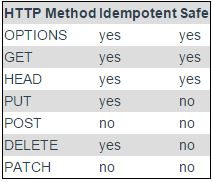
\includegraphics[width=0.5\linewidth]{fig/rest-methods}
\caption{HTTP-Methods}
\label{fig:rest-methods}
\end{figure}